Le jeu de fléchettes oppose deux joueurs et une partie se déroule en plusieurs manches. Les joueurs débutent les manches à tour de rôle. On désigne à pile ou face, avec une pièce équilibrée, la personne qui débute la première manche.

On a étudié les parties entre Pierre et Vanessa et on a constaté que lorsque Pierre joue en premier, il gagne la manche 2 fois sur 3 et lorsqu'il joue en second, il gagne la manche 2 fois sur 5.

On note les évènements :
\begin{itemize}[left=5mm,label={}]
	\item $A$ : \og Pierre joue la manche en premier \fg{} ;
	\item $\overline{A}$ : \og Pierre joue la manche en second \fg{} ;
	\item $G$ : \og Pierre gagne la manche \fg{} ;
	\item $\overline{G}$ : \og Pierre perd la manche \fg.
\end{itemize}

\emph{Pour un évènement quelconque $E$, on note $P(E)$ la probabilité de $E$ et $P_F(E)$ la probabilité de $E$ sachant l'évènement $F$.}

Dans toute la suite, on s'intéresse à la première manche de la partie.

\begin{enumerate}
	\item Recopier et compléter l'arbre de probabilités correspondant :

	\begin{center}
		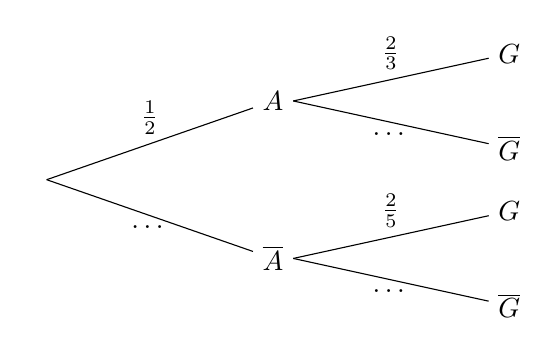
\begin{tikzpicture}[x=3cm, y=1cm]
			
			\node (root) at (0,0) {};
			\node (A) at (1,1) {$A$};
			\node (Abar) at (1,-1) {$\overline{A}$};
			\node (B1) at (2,1.6) {$G$};
			\node (B1b) at (2,0.4) {$\overline{G}$};
			\node (B2) at (2,-0.4) {$G$};
			\node (B2b) at (2,-1.6) {$\overline{G}$};
			
			\draw (root.east) -- (A) node[pos=0.5,above] {$\frac{1}{2}$};
			\draw (root.east) -- (Abar) node[pos=0.5,below] {\ldots};
			
			\draw (A.east) -- (B1) node[pos=0.5,above] {$\frac{2}{3}$};
			\draw (A.east) -- (B1b) node[pos=0.5,below] {\ldots};
			\draw (Abar.east) -- (B2) node[pos=0.5,above] {$\frac{2}{5}$};
			\draw (Abar.east) -- (B2b) node[pos=0.5,below] {\ldots};
		\end{tikzpicture}
	\end{center}

	\item Donner $P_A(G)$ et $P_{\overline{A}}(G)$.
	\item Calculer $P(A \cap G)$. Interpréter cette probabilité dans le contexte de l'exercice.
\end{enumerate}
